%!TEX root = ../../TeseDoutoramento.tex

Lorem ipsum dolor sit amet, consectetur adipiscing elit. Fusce sodales mauris a enim sollicitudin efficitur. Vestibulum et posuere nulla, non luctus mi. Phasellus at condimentum purus. Fusce eget fermentum quam. Donec vel purus tempor, posuere elit non, dignissim justo. Integer vel aliquam nisl. Nulla tincidunt dolor est, quis ultricies neque dapibus at. Donec volutpat elit eget enim volutpat hendrerit. Phasellus id est at est iaculis rhoncus. Nunc rhoncus nisl quis diam feugiat iaculis. Nam nec diam tempus, maximus ante vel, finibus ex. Nunc consequat mattis condimentum. Suspendisse quis neque ac dolor ultricies laoreet. Maecenas sed lacinia enim.


\section{Research data management in the long tail} % (fold)
\label{sec:research_data_management_in_the_long_tail}

Lorem ipsum dolor sit amet, consectetur adipiscing elit. Fusce sodales mauris a enim sollicitudin efficitur. Vestibulum et posuere nulla, non luctus mi. Phasellus at condimentum purus. Fusce eget fermentum quam. Donec vel purus tempor, posuere elit non, dignissim justo. Integer vel aliquam nisl. Nulla tincidunt dolor est, quis ultricies neque dapibus at. Donec volutpat elit eget enim volutpat hendrerit. Phasellus id est at est iaculis rhoncus. Nunc rhoncus nisl quis diam feugiat iaculis. Nam nec diam tempus, maximus ante vel, finibus ex. Nunc consequat mattis condimentum. Suspendisse quis neque ac dolor ultricies laoreet. Maecenas sed lacinia enim.

% section research_data_management_in_the_long_tail (end)

\section{Motivation} % (fold)
\label{sec:motivation}

Lorem ipsum dolor sit amet, consectetur adipiscing elit. Fusce sodales mauris a enim sollicitudin efficitur. Vestibulum et posuere nulla, non luctus mi. Phasellus at condimentum purus. Fusce eget fermentum quam. Donec vel purus tempor, posuere elit non, dignissim justo. Integer vel aliquam nisl. Nulla tincidunt dolor est, quis ultricies neque dapibus at. Donec volutpat elit eget enim volutpat hendrerit. Phasellus id est at est iaculis rhoncus. Nunc rhoncus nisl quis diam feugiat iaculis. Nam nec diam tempus, maximus ante vel, finibus ex. Nunc consequat mattis condimentum. Suspendisse quis neque ac dolor ultricies laoreet. Maecenas sed lacinia enim.


\begin{figure*}
  \begin{center}
    \leavevmode
  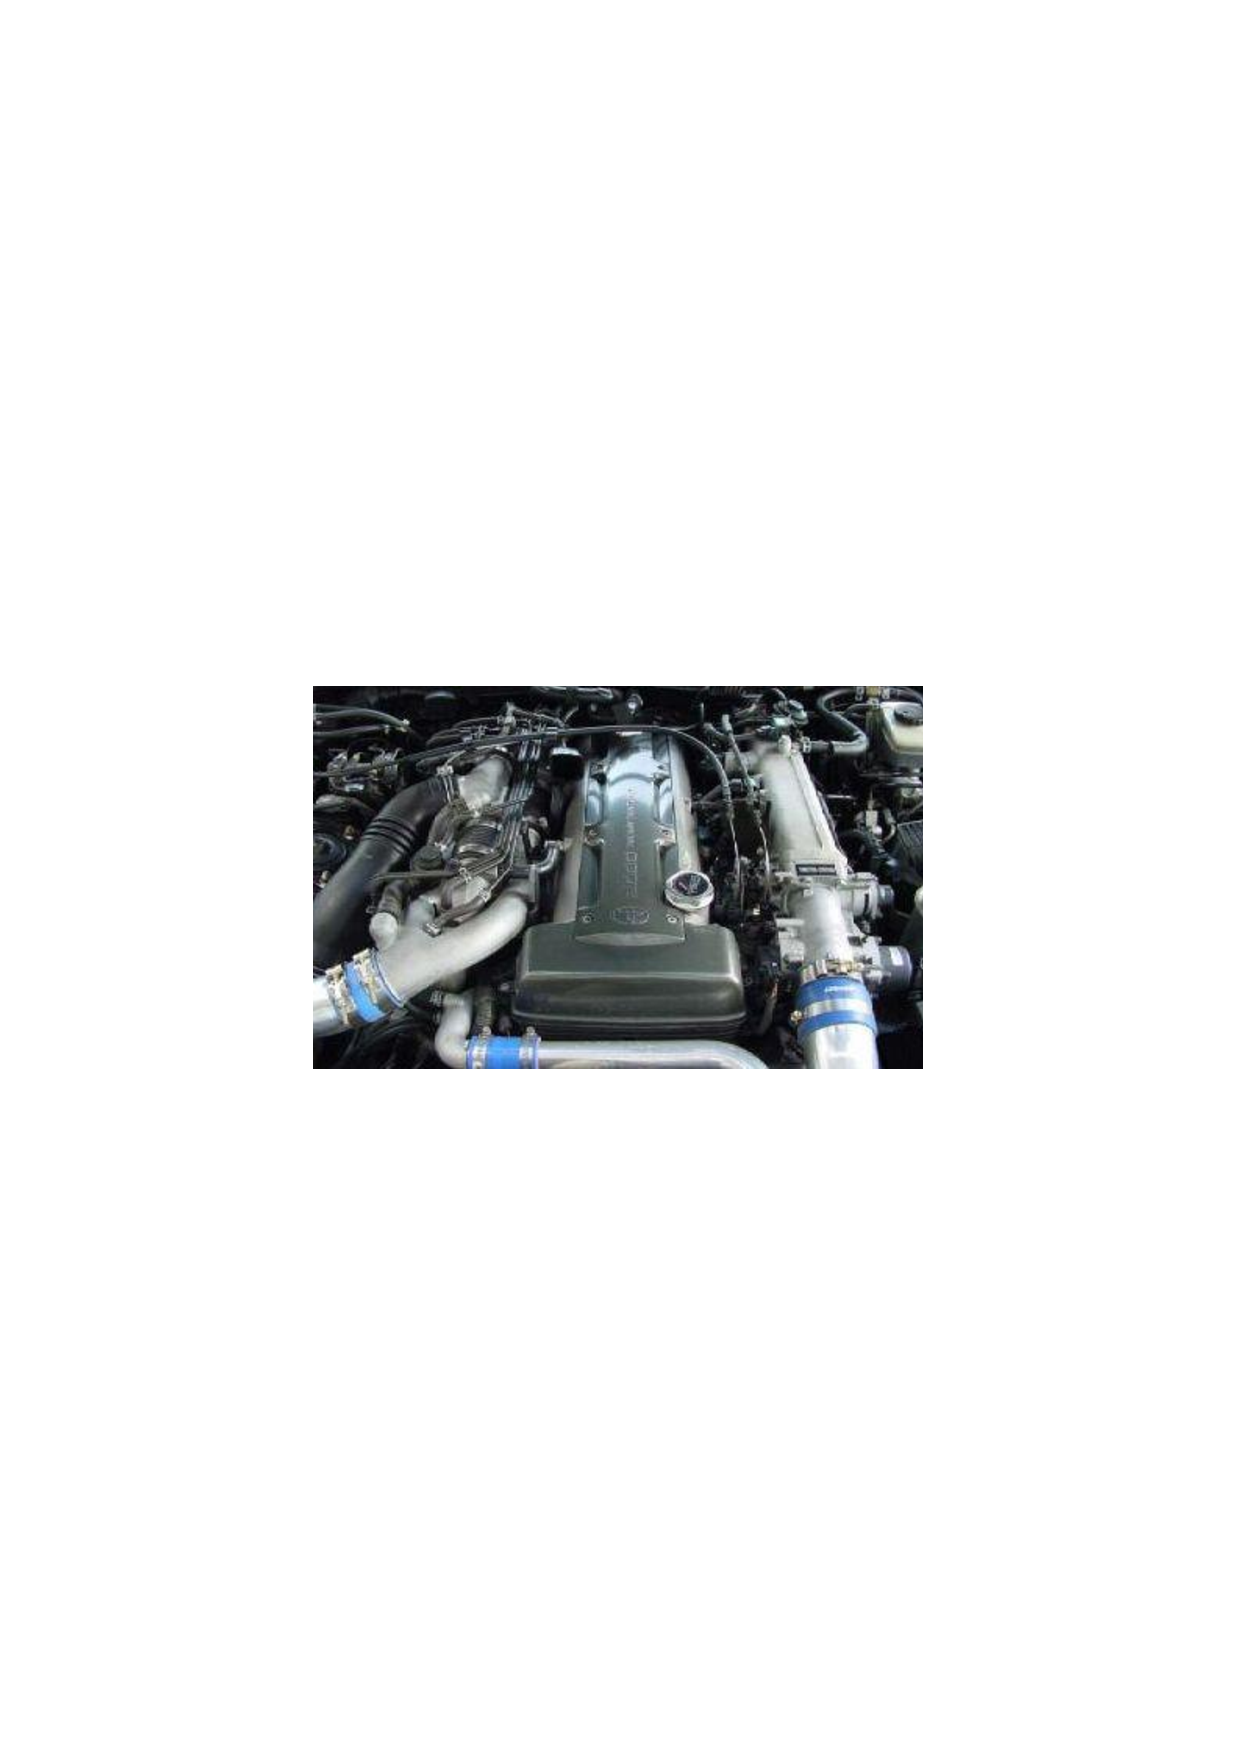
\includegraphics[width=0.9\textwidth]{Images/MK4_supra_engine_bay}
    \caption{An outline of the experiment}
    \label{fig:experiment_outline}
  \end{center}
\end{figure*}

% section motivation (end)

\section{Goals and contributions} % (fold)
\label{sec:goals_and_contributions}

Orci varius natoque penatibus et magnis dis parturient montes, nascetur ridiculus mus. Sed convallis, magna et varius ornare, ligula massa interdum lacus, sed consequat lectus sapien et urna. Donec eu maximus elit, sit amet finibus diam. Curabitur et tincidunt erat, in tincidunt nunc. Ut dapibus auctor ante, in aliquam tortor vehicula tristique. Nam ullamcorper ac magna ac efficitur. Phasellus a lectus at nisi volutpat viverra. Sed id lorem nec eros viverra blandit. Nullam diam turpis, bibendum eu ex vel, hendrerit faucibus nisi. In lorem lorem, gravida eu velit ut, aliquam dapibus lorem. Morbi interdum lectus eu turpis sodales, condimentum lobortis massa sollicitudin. Nulla consectetur dolor ac arcu tempus, ac accumsan tortor efficitur. Maecenas a pretium lacus, nec auctor lorem. Donec sit amet leo ex. Nulla non augue odio. Ut vehicula dignissim massa sed gravida.

\begin{thesisstatement}
The introduction of more silicate to a rubber compound increases the opacity of tire smoke when tire-tarmac friction is applied by a high horsepower vehicle.
\label{hypothesis}
\end{thesisstatement}

Nam rhoncus interdum tellus nec malesuada. Mauris scelerisque tortor in tellus feugiat, commodo pulvinar purus congue. Integer vitae orci et nibh dictum sagittis a sed elit. In commodo arcu nec neque bibendum, ut euismod augue finibus. Morbi efficitur commodo augue quis feugiat. Fusce scelerisque, velit vel ullamcorper tempus, odio erat vehicula urna, non vehicula ligula leo ac magna. Proin non quam tincidunt erat vehicula aliquam tincidunt vitae massa.

\begin{researchquestion}
Which engine has the highest peak horsepower? 2JZ Single Turbo or Twin Turbo?
\label{rq_1_can_collaborative_rdm_environment_engage_researchers}
\end{researchquestion}

\begin{researchquestion}
Can a tire withstand more than 3 laps around a circuit in constant drift?
\label{rq_2_can_usage_information_be_used_to_provide_adequate_recommendations}
\end{researchquestion}

\begin{researchquestion}
Can a 2JZ-GTE be tuned to 500+ hp on stock internals?
\label{rq_3_can_researchers_produce_good_metadata_records_when_supported}
\end{researchquestion}

These research questions are a separation of the hypothesis into sub-problems. Research question ~\ref{rq_1_can_collaborative_rdm_environment_engage_researchers} aims to determine if researchers are willing to carry out a collaborative description effort over their own data, which is what we want to foster with this work. Research question~\ref{rq_2_can_usage_information_be_used_to_provide_adequate_recommendations} covers the means through which we prove our hypothesis: a descriptor recommendation system supported on actual usage information.
%
Finally, research question~\ref{rq_3_can_researchers_produce_good_metadata_records_when_supported} aimed to determine if the quality of the metadata records remains satisfactory after the introduction of the recommendation approach proposed in our work.

Several masters' thesis stemmed from the work on this Ph.D. They are listed as follows:

\begin{itemize}
	\item ``List of masters thesis (full citation)''
\end{itemize}

% section sec:goals_and_contributions (end)

\section{Dissertation structure} % (fold)
\label{sec:dissertation_structure}

This dissertation is organized as follows: ....

% section dissertation_structure (end)